%% ****** Start of file apstemplate.tex ****** %
%%
%%
%%   This file is part of the APS files in the REVTeX 4 distribution.
%%   Version 4.1r of REVTeX, August 2010
%%
%%
%%   Copyright (c) 2001, 2009, 2010 The American Physical Society.
%%
%%   See the REVTeX 4 README file for restrictions and more information.
%%
%
% This is a template for producing manuscripts for use with REVTEX 4.0
% Copy this file to another name and then work on that file.
% That way, you always have this original template file to use.
%
% Group addresses by affiliation; use superscriptaddress for long
% author lists, or if there are many overlapping affiliations.
% For Phys. Rev. appearance, change preprint to twocolumn.
% Choose pra, prb, prc, prd, pre, prl, prstab, prstper, or rmp for journal
%  Add 'draft' option to mark overfull boxes with black boxes
%  Add 'showpacs' option to make PACS codes appear
%  Add 'showkeys' option to make keywords appear
%\documentclass[aps,prl,twocolumn,groupedaddress]{revtex4-1}
\documentclass[%
%reprint,
%superscriptaddress,
%groupedaddress,
%unsortedaddress,
%runinaddress,
%frontmatterverbose, 
twocolumn,
showpacs,preprintnumbers,
%nofootinbib,
%nobibnotes,
%bibnotes,
% amsmath,
 %amssymb,
 aps,
%pra,
%prb,
%rmp,
prstab,
%prstper,
%floatfix,
]{revtex4-1}
%\documentclass[aps,prl,preprint,superscriptaddress]{revtex4-1}
%\documentclass[aps,prl,reprint,groupedaddress]{revtex4-1}

% You should use BibTeX and apsrev.bst for references
% Choosing a journal automatically selects the correct APS
% BibTeX style file (bst file), so only uncomment the line
% below if necessary.
%\bibliographystyle{apsrev4-1}


\usepackage{graphics} % for pdf, bitmapped graphics files
\usepackage[pdftex]{graphicx}
\usepackage{epstopdf}
\usepackage[cmex10]{amsmath}
%\interdisplaylinepenalty=2500
\usepackage{amssymb}  % assumes amsmath package installed
%\usepackage{enumerate}
%\usepackage{setspace}
%\usepackage{verbatim}
\usepackage[colorlinks,linkcolor=blue,pdfauthor=Alexander \ Scheinker,citecolor=red]{hyperref}
%\usepackage{hyperref}


\newtheorem{example}{Example}
\newtheorem{theorem}{Theorem}
\newtheorem{lemma}{Lemma}
\newtheorem{remark}{Remark}
\newtheorem{note}{Note}
\newtheorem{proof}{Proof}

\newtheorem{proposition}{Proposition}
\newtheorem{definition}{Definition}%{definition}
\newtheorem{assumption}{Assumption}
\newtheorem{corollary}{Corollary}%[section]

\begin{document}

% Use the \preprint command to place your local institutional report
% number in the upper righthand corner of the title page in preprint mode.
% Multiple \preprint commands are allowed.
% Use the 'preprintnumbers' class option to override journal defaults
% to display numbers if necessary
%\preprint{}

%Title of paper
\title{Bunch-Length Prediction at the Facility for Advanced Accelerator Experimental Tests (FACET)}

% repeat the \author .. \affiliation  etc. as needed
% \email, \thanks, \homepage, \altaffiliation all apply to the current
% author. Explanatory text should go in the []'s, actual e-mail
% address or url should go in the {}'s for \email and \homepage.
% Please use the appropriate macro foreach each type of information

% \affiliation command applies to all authors since the last
% \affiliation command. The \affiliation command should follow the
% other information
% \affiliation can be followed by \email, \homepage, \thanks as well.
\author{Spencer~Gessner}
\email[]{sgess@slac.stanford.edu}
\author{Alexander~Scheinker}
\email[]{ascheink@lanl.gov}
\thanks{This research was supported by Stanford Linear Accelerator Center and Los Alamos National Laboratory.}
\affiliation{Stanford Linear Accelerator Center}
\affiliation{Los Alamos National Laboratory}

%Collaboration name if desired (requires use of superscriptaddress
%option in \documentclass). \noaffiliation is required (may also be
%used with the \author command).
%\collaboration can be followed by \email, \homepage, \thanks as well.
%\collaboration{}
%\noaffiliation

\date{\today}

\begin{abstract}
In this paper we report on an experiment performed at the Facility for Advanced Accelerator Experimental Tests (FACET), which is the first 2 kilometers of the SLAC Linac, in which a new, model independent adaptive control scheme, rotation rate tuning, was utilized in order to provide a real time bunch length estimate of the beam. The approach was to simultaneously tune many simulation parameters, such as arbitrary phase shifts, in order to match a simulated (LiTrack) bunch energy spread spectrum with the real time wiggler/ scintillating YAG crystal signal. The simple adaptive scheme was digitally implemented using Matlab and the Experimental Physics and Industrial Control System (EPICS). The main result is the development of a non-intrusive, non-destructive real-time diagnostic scheme for prediction of bunch length, as well as other beam parameters, the precise control of which is very important for the plasma acceleration scheme being explored at FACET.
\end{abstract}

% insert suggested PACS numbers in braces on next line
\pacs{41.85.Lc, 02.30.Yy, 29.20.-c, 02.60.-x}
% insert suggested keywords - APS authors don't need to do this
%\keywords{}

%\maketitle must follow title, authors, abstract, \pacs, and \keywords
\maketitle





%%%%%%%%%%%%%%%%%%%%%%%%%%%%%%%%%%%%%%%%%%%%%%%%%%%%%%%%%%%%%%%%%%%%%%%%%%%%%%%%%%%%%%%%

%%%%%%%%%%%%%%%%%%%%%%%%%%%%%%%%%%%%%%%%%%%%%%%%%%%%%%%%%%%%%%%%%%%%%%%%%%%%%%%%%%%%%%%%

\section{Introduction}

%%%%%%%%%%%%%%%%%%%%%%%%%%%%%%%%%%%%%%%%%
\subsection{Motivation}
%%%%%%%%%%%%%%%%%%%%%%%%%%%%%%%%%%%%%%%%%

The Facility for Advanced Accelerator Experimental Tests (FACET) at SLAC produces high energy electron beams for Plasma Wakefield Acceleration. For these experiments, precise measurement and control of the longitudinal beam profile is very important. A number of bunch length diagnostics are employed at FACET, including beam streaking with an x-band transverse deflecting cavity (TCAV) \cite{ref-FACET}. A non destructive bunch-length measurement, along with the results of a plasma acceleration event from the measured beam, would provide valuable data, and feedback to machine operators, so that real-time adjustments can be made, in order to make sure that the beam has the desired properties.

Because of the complexity of FACET, including nonlinear dynamics of intense electron bunches traveling through a two kilometer particle accelerator, uncertainty of arbitrary phase shifts, and time-varying coupling between many components, it is impossible to write down an analytic machine settings to bunch length formula. Even if such a formula was available, the uncertainty and time variation of parameters would make this model imperfect. Therefore, a model independent scheme was proposed, which could adaptively tune unknown parameter settings, in order to match a simulated LiTrack spectrum to the TCAV spectrum measured in the actual machine. The hope was that by matching machine and simulation spectra, a beam property such as bunch length could be predicted, in real time, without destructive beam measurement.




%%%%%%%%%%%%%%%%%%%%%%%%%%%%%%%%%%%%%%%%%
\subsection{Results of the paper}
%%%%%%%%%%%%%%%%%%%%%%%%%%%%%%%%%%%%%%%%%

We developed a real-time, non-destructive diagnostic for bunch length prediction, by combining the adaptive rotation rate (RR) \cite{ref-stab-sch} method, with the LiTrack simulation of the beam, and the real time, non-destructive TCAV spectrum. We simulated FACET with fourteen free parameters in a code package called LiTrackES. The adaptive scheme worked by minimizing a cost, which was the $\chi^2$ residual between the measured (TCAV) and simulated (LiTrack) spectra of the electron bunch. System parameters such as various arbitrary phase shifts and beam properties ($\beta$, dispersion) were the inputs to LiTrack, the adaptive scheme minimized the cost by varying all of these parameters simultaneously, in order to match the code's spectrum to that measured in the machine and to track time-varying properties of the beam due to machine parameter changes.

%%%%%%%%%%%%%%%%%%%%%%%%%%%%%%%%%%%%%%%%%
\subsection{Organization} 
%%%%%%%%%%%%%%%%%%%%%%%%%%%%%%%%%%%%%%%%%

In Section~\ref{sec:facet} we give a brief overview of FACET and the importance of bunch length and other beam properties on plasma acceleration dynamics. In Section \ref{sec:litrack} we give an overview of the LiTrack software used to simulate the accelerator, as a virtual, real time observer of the actual electron bunch. In Section \ref{sec:tune} we provide background and an overview of the adaptive method used. Finally, in Section \ref{sec:results} we present our main results.



%%%%%%%%%%%%%%%%%%%%%%%%%%%%%%%%%%%%%%%%%%%%%%%%%%%%%%%%%%%%%%%%%%%%%%%%%%%%%%%%%%%%%%%%

%%%%%%%%%%%%%%%%%%%%%%%%%%%%%%%%%%%%%%%%%%%%%%%%%%%%%%%%%%%%%%%%%%%%%%%%%%%%%%%%%%%%%%%%

\section{Overview of FACET}\label{sec:facet}



%%%%%%%%%%%%%%%%%%%%%%%%%%%%%%%%%%%%%%%%%
\subsection{Machine Layout}
%%%%%%%%%%%%%%%%%%%%%%%%%%%%%%%%%%%%%%%%%




%%%%%%%%%%%%%%%%%%%%%%%%%%%%%%%%%%%%%%%%%
\subsection{Bunch Shape Influence on Plasma Acceleration}
%%%%%%%%%%%%%%%%%%%%%%%%%%%%%%%%%%%%%%%%%




%%%%%%%%%%%%%%%%%%%%%%%%%%%%%%%%%%%%%%%%%%%%%%%%%%%%%%%%%%%%%%%%%%%%%%%%%%%%%%%%%%%%%%%%

%%%%%%%%%%%%%%%%%%%%%%%%%%%%%%%%%%%%%%%%%%%%%%%%%%%%%%%%%%%%%%%%%%%%%%%%%%%%%%%%%%%%%%%%

\section{Li-Track}\label{sec:litrack}

%%%%%%%%%%%%%%%%%%%%%%%%%%%%%%%%%%%%%%%%%%%%%%%%%%%%%%%%%%%%%%%%%%%%%%%%%%%%%%%%%%%%%%%%

%%%%%%%%%%%%%%%%%%%%%%%%%%%%%%%%%%%%%%%%%%%%%%%%%%%%%%%%%%%%%%%%%%%%%%%%%%%%%%%%%%%%%%%%

\section{Adaptive Tuning Method}\label{sec:tune}

\begin{figure}[!t]
\centering
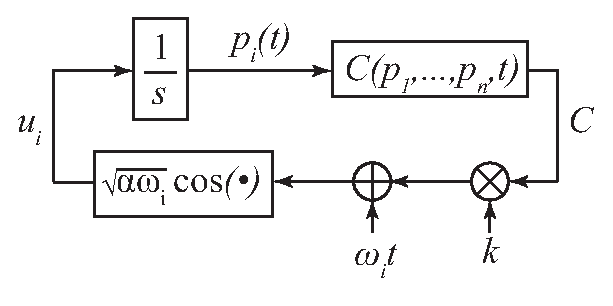
\includegraphics[width=.35\textwidth]{f2}
\caption{Tuning of the $i^{th}$ component  $p_i$ of $\mathbf{p} = (p_1, \dots, p_n) \in \mathbb{R}^n$. The symbol $\frac{1}{s}$ denotes the Laplace Transform of an integrator, so that in the above diagram $p_i(t) = p_i(0)+ \int_{0}^{t} u_i(\tau)d\tau$.}
\label{fig:th1}
\end{figure}

\begin{figure*}[!t] 
    \centering
    \includegraphics[width=.98\textwidth]{FACET2}
    \caption{The actual FACET accelerator (a) is run along with the LiTrack simulator (b), whose initial parameter inputs, $p_i(0)$, are a combination of accurately measured settings and guesses for time-varying, not easily detectable actual settings, such as drifting RF phase. The measured and predicted YAG spectrums are compared (c) and a cost, $C(n+1)$ is calculated based on the mismatch. The cost is fed into the adaptive scheme (d), as described above, and the parameters are automatically tuned and updated (e). When the cost is oscillating near minimum, the bunch length prediction is most accurate (f).}
    \label{fig:ltes}
\end{figure*}

\begin{figure}[!t] 
    \centering
    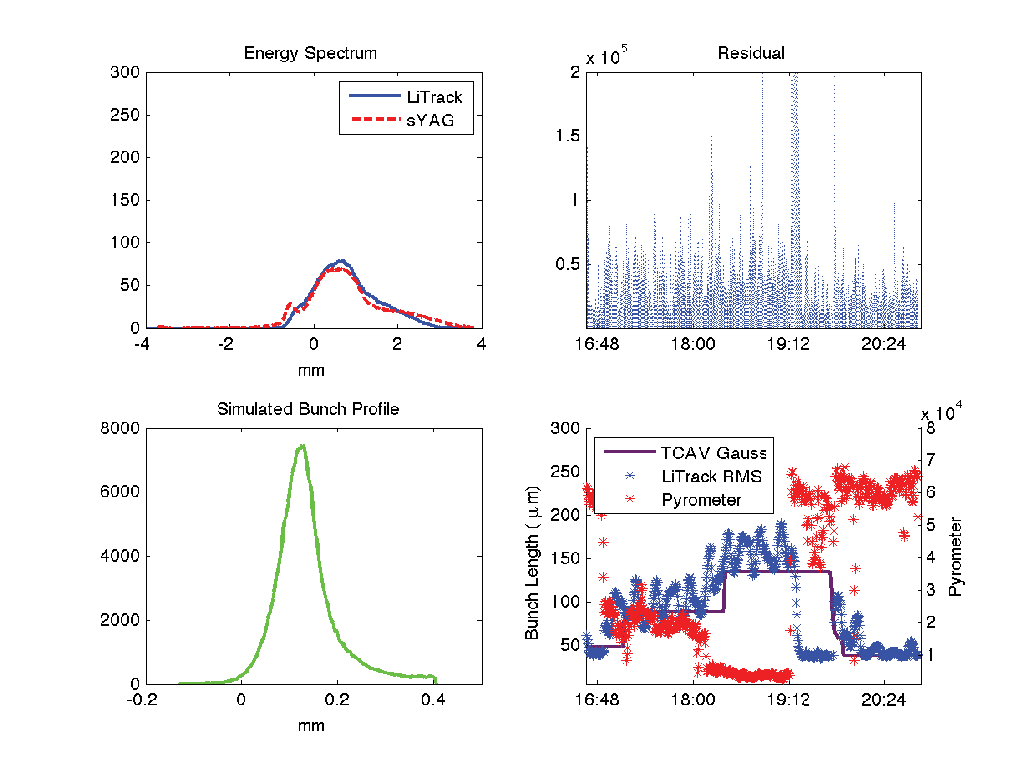
\includegraphics[width=.45\textwidth]{f3}
    \caption{Comparison of LiTrackES with TCAV and Pyrometer over a four hour period. Note that the pyrometer varies inversely with bunch length.}
    \label{fig:fc}
\end{figure}


\begin{figure*}[!t] 
    \centering
    \includegraphics[width=.98\textwidth]{3D_All}
    \caption{The LiTrack spectrum (green) is shown converging to the measured spectrum (black), as the scaled parameters (top) find optimal values, while remaining within their constraints (red/dashed), over 1800 iterations. The cost approaches a minimum as the spectrums become matched. Once the cost is sufficiently small and therefore the spectrum match is sufficiently accurate, we trust the bunch length prediction. As accelerator and beam properties change, the adaptive scheme stays locked-on to the machines time-varying spectrum, thereby tracking time-varying beam properties.}
    \label{fig:spectconv}
\end{figure*}

For complex systems, with nonlinear coupling between many components, such as particle accelerators, sophisticated, multidimensional, nonlinear optimization schemes, such as genetic algorithms (GA) \cite{ref-GA-1} are powerful tools for aiding in the design process. GAs have been successfully used for photoinjector design \cite{ref-GA-2}, damping ring design \cite{ref-GA-25}, storage ring dynamics \cite{ref-GA-275}, global optimization of a lattice \cite{ref-GA-3}, neutrino factory design \cite{ref-GA-4}, simultaneous optimization of beam emittance and dynamic aperture \cite{ref-GA-5}, and free electron laser linac drivers \cite{ref-GA-6}. A review of many GA applications for accelerator physics is given in \cite{ref-GA-7}.

One limitation, however, of GAs is their model-dependence. In the face of coupling, nonlinearities, and most importantly, model uncertainty, a model independent, feedback-based adaptive scheme is required. The adaptive feedback tuning method that we used is the rotation rate (RR) method, which is described in detail in \cite{ref-stab-sch}. Here, we briefly recall (RR) and it's implementation.

For our problem, we vary, in simulation, the parameters:
\begin{itemize}
	\item $p_1$: Phase of the Klystron in sector \cite{?}
	\item $p_2$: \cite{?}
	\item $p_3$: \cite{?} \\ \vdots
\end{itemize}

Each parameter setting had its own influence on electron bunch dynamics, which in turn influenced the separation, amount of charge in, emmitance, length, .... , of the leading and trailing electron bunches. Bunch properties correlated to an energy spectrum which was detected in the transverse deflecting cavity. The cost that our adaptive scheme was attempting to minimize was then the difference between the actual, detected spectrum, and that predicted by LiTrack:

\begin{equation}
	C(\mathbf{p}(n),t) = \int \left | \psi(f,t) - \hat{\psi}(f,\mathbf{p}(n)) \right |^2 df,
\end{equation}
in which $\psi(f,t)$ was the actual, time-varying (due to phase drift, thermal cycling...) detected spectrum, and $\hat{\psi}(f,\mathbf{p}(n))$ was the LiTrack, simulated spectrum, which depends on parameter settings $\mathbf{p}(n)$.


The problem was then to locate the minimum of the function $C(\mathbf{p},t):\mathbb{R}^n\times \mathbb{R}^+ \rightarrow \mathbb{R}$, for $\mathbf{p} = (p_1, \dots, p_n) \in \mathbb{R}^n$, which we can measure the value of, but whose analytic form is unknown. The hope was that, by finding simulation machine settings which resulted in matched spectrums, we would also match other properties of the real and simulated beams, such as bunch length, something we could not simply do by setting the simulation parameters to the exact machine settings, due to unknowns, such as time-varying, arbitrary phase shifts.

The first step of the adaptive scheme was to choose physically realizable constraints for all parameters:
\begin{eqnarray}
	\mathbf{p}_{\mathrm{max}} &=& \left ( p_{1,\mathrm{max}}, \dots, p_{m,\mathrm{max}} \right ), \mathbf{p}_{\mathrm{min}} = \left (  p_{1,\mathrm{min}}, \dots, p_{m,\mathrm{min}} \right ). \nonumber
\end{eqnarray}
Implementing initial parameter settings $\mathbf{p}(1)$, which are chosen based on the physics model and experience, allowed us to calculate $C(\mathbf{p}(1))$. The iterative update scheme was then:
\begin{equation}
	p_i(n+1) = p_i(n) + \Delta \sqrt{\alpha\omega_i}\cos \left ( \omega_i n \Delta + k C(\mathbf{p}(n)) \right ), \label{ESschm}
\end{equation}
which is based on the finite difference approximation of the derivative:
\begin{equation}
	\frac{p_i(t+\Delta)-p_i(t)}{\Delta} \approx \frac{\partial p_i}{\partial t} = \sqrt{\alpha\omega_i}\cos \left ( \omega_i t + k C(\mathbf{p}(t),t) \right ), \label{ESschmdr}
\end{equation}
which we may expand as
\begin{equation}
\cos \left (\omega_i t + kC \right ) = \cos(\omega_i t)\cos\left (kC \right ) - \sin \left (\omega_i t \right )\sin \left (kC \right )
\end{equation}
and rewrite the $p_{i}$ $\left ( 1 \leq i \leq n \right )$ dynamics as
\begin{equation}
	\dot{p}_{i} = \sqrt{\omega_i}\cos(\omega_i t)\sqrt{\alpha}\cos \left (k C \right )  -\sqrt{\omega_i}\sin(\omega_i t)\sqrt{\alpha}\sin\left (k C \right),
\end{equation}
which, according to the results of \cite{ref-stab-sch}, resulted in an average parameter and cost relationship of the form:
\begin{eqnarray}
	\dot{\bar{p}}_{i} &=& -\frac{k \alpha}{2} \frac{\partial C\left ( \bar{\mathbf{p}},t\right )}{\partial \bar{p}_{i}}\left ( \cos^2 \left (k C\left ( \bar{\mathbf{p}},t\right ) \right ) + \sin^2 \left (k C\left ( \bar{\mathbf{p}},t\right ) \right ) \right ) \nonumber \\
	&=& -\frac{k \alpha}{2} \frac{\partial C\left ( \bar{\mathbf{p}},t\right )}{\partial \bar{p}_{i}},
\end{eqnarray}
and therefore
\begin{equation}
	\dot{\bar{\mathbf{p}}} = -\frac{k \alpha}{2} \mathbf{\nabla C},
\end{equation}
which is a gradient descent towards the minimum of $C$.

The constraints were simply implemented by checking the updated parameters at each step and confining them to their bounds if necessary:
\begin{align*}
	&\mathrm{ \bf IF} \ p_i(n+1)>p_{i,\mathrm{max}},  &&\mathrm{\bf THEN} \ p_i(n+1)=p_{i,\mathrm{max}}, \nonumber \\
	&\mathrm{ \bf IF} \ p_i(n+1)<p_{i,\mathrm{min}},  &&\mathrm{\bf THEN} \ p_i(n+1)=p_{i,\mathrm{min}}. \nonumber
\end{align*}

Because the values of different parameters $p_i$ differed by orders of magnitude, they each required individual values of $k_i$ and $\alpha_i$. Therefore, we normalized the parameters to within $[-1,1]$ bounds. At each step $n$, the cost $C(n)$ was computed based on parameter settings $\mathbf{p}(n)$, then translate into the scaled parameters $\mathbf{p}_{s}(n)$:
\begin{equation}
	p_{\mathrm{s},i}(n) =  \frac{ 2\left ( p_i(n) - C_{p,i} \right ) }{D_{p,i}},
\end{equation}
where $C_{p,i}=\frac{p_{i,\mathrm{max}}+p_{i,\mathrm{min}}}{2}$ and $D_{p,i} = p_{i,\mathrm{max}} - p_{i,\mathrm{min}}$, bounding each parameter within $[-1,1]$. We then performed the RR-update on the scaled parameters
\begin{equation}
	p_{s,i}(n+1) = p_{s,i}(n) + \Delta \sqrt{\alpha_i\omega_i}\cos \left ( \omega_i n \Delta + k_i C(\mathbf{p}(n)) \right ),
\end{equation}
while forcing the scaled parameters to satisfy the constraints $-1$ and $1$. Finally, we transformed back into un-scaled parameter values in order to calculate the cost for the next iteration:
\begin{equation}
	p_i(n+1) =  \frac{p_{s,i}(n+1)D_{p,i}}{2} + C_{p,i}.
\end{equation}


%%%%%%%%%%%%%%%%%%%%%%%%%%%%%%%%%%%%%%%%%%%%%%%%%%%%%%%%%%%%%%%%%%%%%%%%%%%%%%%%%%%%%%%%

%%%%%%%%%%%%%%%%%%%%%%%%%%%%%%%%%%%%%%%%%%%%%%%%%%%%%%%%%%%%%%%%%%%%%%%%%%%%%%%%%%%%%%%%

\section{Results}\label{sec:results}

The algorithm and LiTrack were initialized with parameters that are assumed to be close to the real machine parameters. In general, the initial guess does not provide an accurate estimate of the measured energy spectrum, but the adaptive scheme evolves the simulation parameters to find the match. On average, it took about 500 iterations of the algorithm (roughly 5 minutes) to find a match. Once a match was found, the system was stabilized and remained locked to the measured energy spectrum. LiTrackES was found to be in agreement with the TCAV and pyrometer. The obvious advantage of LiTrackES over the other methods was that LiTrackES provided real time bunch profile. The pyrometer is sensitive to peak current rather than bunch profile and the TCAV cannot be used every shot. The experimental setup is shown in Figure \ref{fig:ltes}. The results of the run are shown in Figure \ref{fig:fc}.

%%%%%%%%%%%%%%%%%%%%%%%%%%%%%%%%%%%%%%%%%%%%%%%%%%%%%%%%%%%%%%%%%%%%%%%%%%%%%%%%%%%%%%%%

%%%%%%%%%%%%%%%%%%%%%%%%%%%%%%%%%%%%%%%%%%%%%%%%%%%%%%%%%%%%%%%%%%%%%%%%%%%%%%%%%%%%%%%%

\section{Conclusions and Future Work} \label{sec:con}


xxxxxxxxx


%%%%%%%%%%%%%%%%%%%%%%%%%%%%%%%%%%%%%%%%%%%%%%%%%%%%%%%%%%%%%%%%%%%%%%%%%%%%%%%%%%%%%%%%

%%%%%%%%%%%%%%%%%%%%%%%%%%%%%%%%%%%%%%%%%%%%%%%%%%%%%%%%%%%%%%%%%%%%%%%%%%%%%%%%%%%%%%%%



\begin{thebibliography}{99}

\bibitem{ref-GA-1} R. Hajima, N. Taked, H. Ohashi, and M. Akiyama, Nucl. Instrum. Methods Phys. Res., Sect. A {\bf 318}, 822 (1992).

\bibitem{ref-GA-2} I. Bazarov and C. Sinclair, Phys. Rev. ST Accel. Beams {\bf 8}, 034202 (2005).

\bibitem{ref-GA-25} L. Emery, Global optimization of damping ring designs using a multi-objective evolutionary algorithm, in: PAC 2005, (2005).

\bibitem{ref-GA-275} M. Borland, V. Sajaev, L. Emery, A. Xiao, ``Direct methods of optimization of storage ring dynamic and momentum aperture," {\it Proc. PAC}, 2009.

\bibitem{ref-GA-3} L. Yang, D. Robin, F. Sannibale, C. Steier, and W. Wan, Nucl. Instrum. Methods Phys. Res., Sect. A {\bf 609}, 50, (2009).

\bibitem{ref-GA-4} A. Poklonskiy and D. Neuffer, Int. Journal. Modern. Phys., A, {\bf 24} 5 (2009).

\bibitem{ref-GA-5} W. Gao, L. Wang, and W. Li, Phys. Rev. ST Accel. Beams {\bf 14}, 094001 (2011).

\bibitem{ref-GA-6} R. Bartolini, M. Apollonio, and I.P.S. Martin, Phys. Rev. ST Accel. Beams {\bf 15}, 030701 (2012).

\bibitem{ref-GA-7} A. Hofler, B. Terzic, M. Kramer, A. Zvezdin, V. Morozov, Y. Roblin, F. Lin, and C. Jarvis, Phys. Rev. ST Accel. Beams {\bf 16}, 010101 (2013).

\bibitem{ref-stab-sch} A. Scheinker, X. Pang, and L. Rybarcyk, Phys. Rev. ST Accel. Beams {\bf 16}, 102803 (2013).

\bibitem{ref-FACET} S. Gessner, E. Adili, F. Decker, M. Hogan, T. Raubenheimer, A. Scheinker, ``Longitudinal phase space dynamics with novel diagnostic techniques at FACET," {\it Proc. IPAC}, 2013.

\end{thebibliography}


\end{document}


